% Section 4: BAA Architecture — revised per supervisor review (2026-08-28)
% Changes: expanded §4.7 with char/river island practical example; 
%          constrained decoding prompt rendered in \texttt monospace; 
%          tier descriptions flow as prose with bold inline headers.

\section{Bounded-Authority Advisory Architecture (BAA)}
\label{sec:system_architecture}

\subsection{Architectural Overview}
BAA is organized as a five-tier selective resolution ladder with a downstream relational verifier (Figure~\ref{fig:architecture}). The core architectural principle is that resolution and verification are deterministic and typed, while generation is strictly a bounded realization step.

\begin{enumerate}
    \item[\textbf{Tier~0}] \textbf{Risk and context gate.} Lightweight deterministic screening for banned/restricted chemicals, poisoning and self-harm framings, and prompt-injection payloads before any retrieval or generation occurs.
    \item[\textbf{Tier~1}] \textbf{Capability and perception router.} Entity normalization across Bengali registers (standard formal, authentic farmer, regional dialects, Banglish) plus optional crop classification from an uploaded image to narrow candidate search spaces.
    \item[\textbf{Tier~2}] \textbf{Structured fact authority and deterministic resolver.} Typed, versioned, provenance-carrying records in a local fact store. A resolver maps $\langle\text{crop}, \text{problem}, \text{stage}, \text{intent}\rangle$ to a fact record and renders a certified answer from a validated template with zero LLM invocation.
    \item[\textbf{Tier~3}] \textbf{Grounded generative realization.} For queries with valid retrieved evidence but no deterministic template match, an instruction-tuned LLM phrases an answer under a single-record constraint contract.
    \item[\textbf{Tier~4}] \textbf{Verification and fail-closed output.} The relational verifier re-derives the candidate tuple from the response and validates it against the single accredited evidence record hash, failing closed to clarify, abstain, or escalate on any discrepancy.
\end{enumerate}

\subsection{Risk/Context Gate}
The gate applies a deterministic, six-way policy classification before any retrieval: \emph{safe\_agri}, \emph{banned\_or\_restricted\_chemical}, \emph{self\_harm\_or\_poisoning\_risk}, \emph{off\_topic}, \emph{prompt\_injection}, and \emph{low\_confidence}. Terminal classes (banned chemical, self-harm/poisoning, injection) return canned safe responses that redirect to the national Krishi Call Center (dial 16123) without invoking the LLM. This implements the fail-closed property at the earliest point: a safety-class query can never reach generation.

\subsection{Capability Router and Entity Normalization}
A lightweight character $n$-gram intent classifier (1.25~MB, p50 latency 0.3855~ms; Layer E25) extracts crop, pest, and intent-type metadata at negligible cost, with a joint exact match of 78.4\% (95\% CI [72.89, 83.05]). Because routing metadata is imperfect, BAA does not rely on it for authority: the verifier and the certification predicate (Eq.~\ref{eq:certification_rule}) absorb routing uncertainty, so a wrong metadata label cannot produce an unsafe certification. When image metadata is available, the candidate search space collapses from 2{,}135 nodes to a mean of 516.4 nodes ($-$75.64\%; Layer E17, threshold 0.8), with a misrouting rate of 3.15\% (95\% CI [2.65, 3.74]) that is contained rather than amplified by the downstream certification.

\subsection{Structured Fact Authority and Deterministic Resolution}
The fact store holds typed records with a 20-field schema (crop, problem, stage, active ingredient, formulation, dose bounds, unit, volume, interval, PHI, regulatory status, source ID, source version, effective/expiry dates, verifier identity, evidence hash). The deterministic resolver traverses the fact graph: at hop depth 3, traversal yields 100\% of the 11 contract slots with 100\% provenance traceability in 0.0128~ms mean latency (Layer E19, 23-node proof-of-mechanism graph). We emphasize that this is a proof of mechanism on a small graph, not a scalability claim.

\subsection{Generative Realization with Constrained Decoding}
When the deterministic path cannot fire but evidence exists, Tier~3 invokes the LLM (a fine-tuned Gemma-4 4-bit model in the local deployment, or an API model in the cloud variant) with the constraint: \texttt{you may explain these facts in Bengali; you must not alter numerical or regulatory fields.} Generation is always followed by the verifier. The architecture deliberately does not ask the LLM to infer missing evidence; missing evidence routes to recovery (re-retrieval, normalization, structured retry) or abstention.

\subsection{Relational Certification and Fail-Closed Execution}
The verifier checks: schema validity, numerical consistency against the record's dosage bounds, unit consistency, formulation compatibility, crop--problem compatibility, temporal validity, source binding (the 11-slot tuple must come from one record hash), and banned/restricted registry status. Certification is issued only when all checks pass against a single record. This is the mechanism that ensures cross-record and counterfactual misbinding are structurally rejected by the certification predicate whenever the contract fields are correctly extracted and the authority record is valid, and it is the mechanism empirically evaluated in Section~\ref{sec:results_authority_safety}.

\subsection{Temporal and Provenance Controls}
Each record carries effective/expiry dates and an authority manifest (Section~\ref{sec:knowledge_governance}). At certification time, the resolver validates the record against the manifest; a superseded record fails the $\operatorname{Current}(e)$ predicate and cannot be certified even if its text is retrieved. Every certified output emits a provenance chain (\texttt{answer claim $\rightarrow$ structured fact $\rightarrow$ source node $\rightarrow$ source document $\rightarrow$ document version/date}).

\subsection{Offline, Edge, and Channel Support}
A signed offline fact pack (SQLite) supports deterministic resolution and verification with zero network access. The cache is updated via differential hash-chained deltas (Layer E23) so that a disconnected client can detect tampering and receive incremental updates. This has a direct practical implication for deployment in Bangladesh: a farmer on a \emph{char} (river island) with no mobile connectivity can still receive a certified pesticide advisory, resolved entirely on-device from the offline fact pack. Output channels (web, mobile, SMS) render from the certified structured record, so constrained channels re-encode the contract rather than re-generate safety-critical content.

\begin{figure*}[pos=t]
\centering
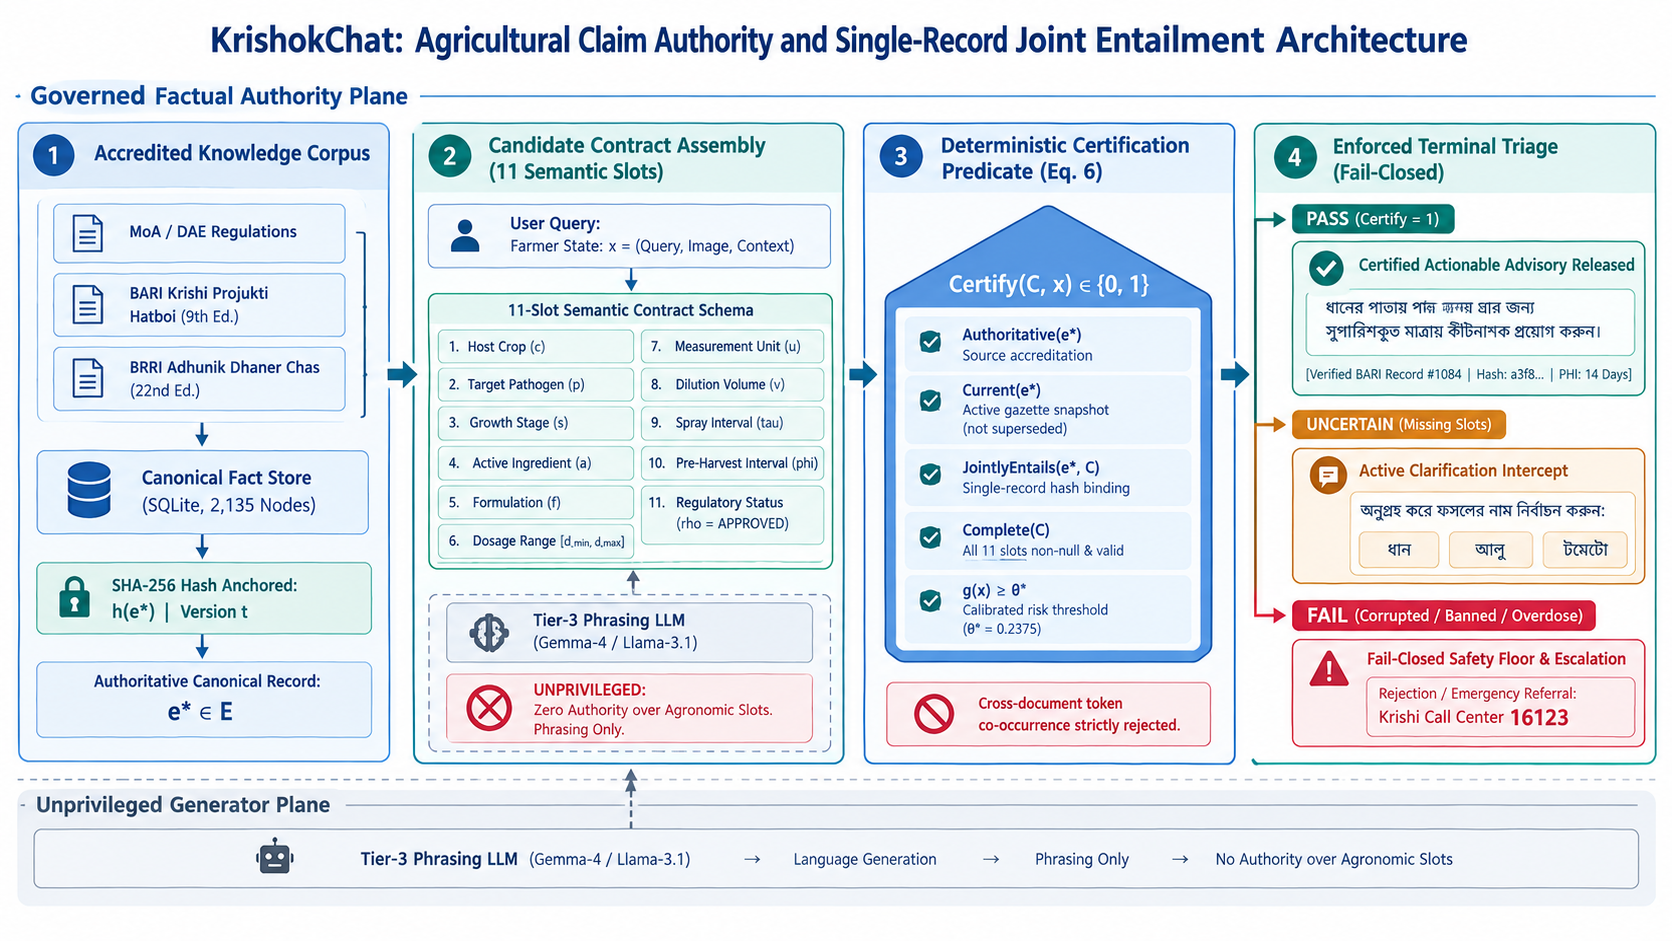
\includegraphics[width=0.92\textwidth,height=7.2cm,keepaspectratio]{figures/fig_1.png}
\caption{The Bounded-Authority Advisory Architecture (BAA). Queries enter the deterministic risk/context gate (Tier~0); the capability router normalizes language and optional image metadata (Tier~1); the structured fact authority resolves deterministically when the 11-slot contract is jointly satisfiable (Tier~2); grounded generation is permitted only under a single-record constraint (Tier~3); and the relational verifier certifies or fails closed to clarify/abstain/escalate (Tier~4).}
\label{fig:architecture}
\end{figure*}